\documentclass[a4paper, 12pt, ngerman]{exam}
\usepackage{preamble/draft}
%\usepackage{polynom}
\usepackage{pgfplots}
\pgfplotsset{compat = newest}
\tikzset{answer/.style={draw,text opacity=0},answer plot/.style={opacity=0}}
\let\oldprintanswers\printanswers
\def\printanswers{\oldprintanswers\tikzset{answer/.style={text opacity=1},
answer plot/.style={opacity=1}}}

% layout for listings
\lstset{
 morekeywords={for, in, if, then, endfor},
 basicstyle=\ttfamily,
 keywordstyle=\bfseries,
 frame=single,
 frameround=tttt,
 escapeinside={|}{|},
 numbers=left,
 numberstyle=\tiny,
 breaklines=true
}

% page layout
\geometry{a4paper,left=2.5cm,right=2.5cm, top=3cm, bottom=3cm}

% font layout
\titleformat{\chapter}[display]
  {\normalfont\sffamily\huge\bfseries}
    {\chaptertitlename\ \thechapter}{20pt}{\Huge}
%\titleformat*{\chapter}{\LARGE\bfseries\sffamily}
\titleformat*{\section}{\Large\bfseries\sffamily}
\titleformat*{\subsection}{\large\bfseries\sffamily}
\titleformat*{\subsubsection}{\normalsize\bfseries\sffamily}
\titleformat*{\paragraph}{\small\bfseries\sffamily}
\titleformat*{\subparagraph}{\footnotesize\bfseries\sffamily}



\newcommand{\examtype}{Übung Differentialrechnung}
\newcommand{\examno}{2}
\newcommand{\examdate}{26.04.2022}
\newcommand{\subject}{Mathematik}
\newcommand{\examclass}{}

%\addpoints
\pointpoints{Punkt}{Punkte}
\bonuspointpoints{Bonuspunkt}{Bonuspunkte}
\renewcommand{\solutiontitle}{\noindent\textbf{Lösung:}%
\enspace}

\chqword{Frage}
\chpgword{Seite}
\chpword{Punkte}
\chbpword{Bonuspunkte}
\chsword{Erreicht}
\chtword{Gesamt}

\hpword{Punkte:} % Punktetabelle
\hsword{Ergebnis:}
\hqword{Aufgabe:}
\htword{Summe:}

\pagestyle{headandfoot}
\firstpageheadrule
\runningheadrule
\firstpageheader{\examclass}{\large{\textbf{\subject}}\\ \large{\examtype\ \examno}}{\examdate}
\runningheader{\examclass}{\large{\textbf{\subject}}\\ \large{\examtype\ \examno}}{\examdate}
\firstpagefooter{}{Seite \thepage\ von \numpages}{}
\runningfooter{}{Seite \thepage\ von \numpages}{}

\qformat{\textbf{Aufgabe \thequestion} \hfill}
\pointformat{}

\pointsinrightmargin

\renewcommand{\familydefault}{\sfdefault}

\colorgrids
\definecolor{GridColor}{gray}{0.7}

\tikzumlset{fill class=white}


%\printanswers

\begin{document}

\begin{questions}
 
  \question
  Gegeben sei folgender Graph der Funktion $f(x) = x^3+2x^2-3$:
  \begin{center}
    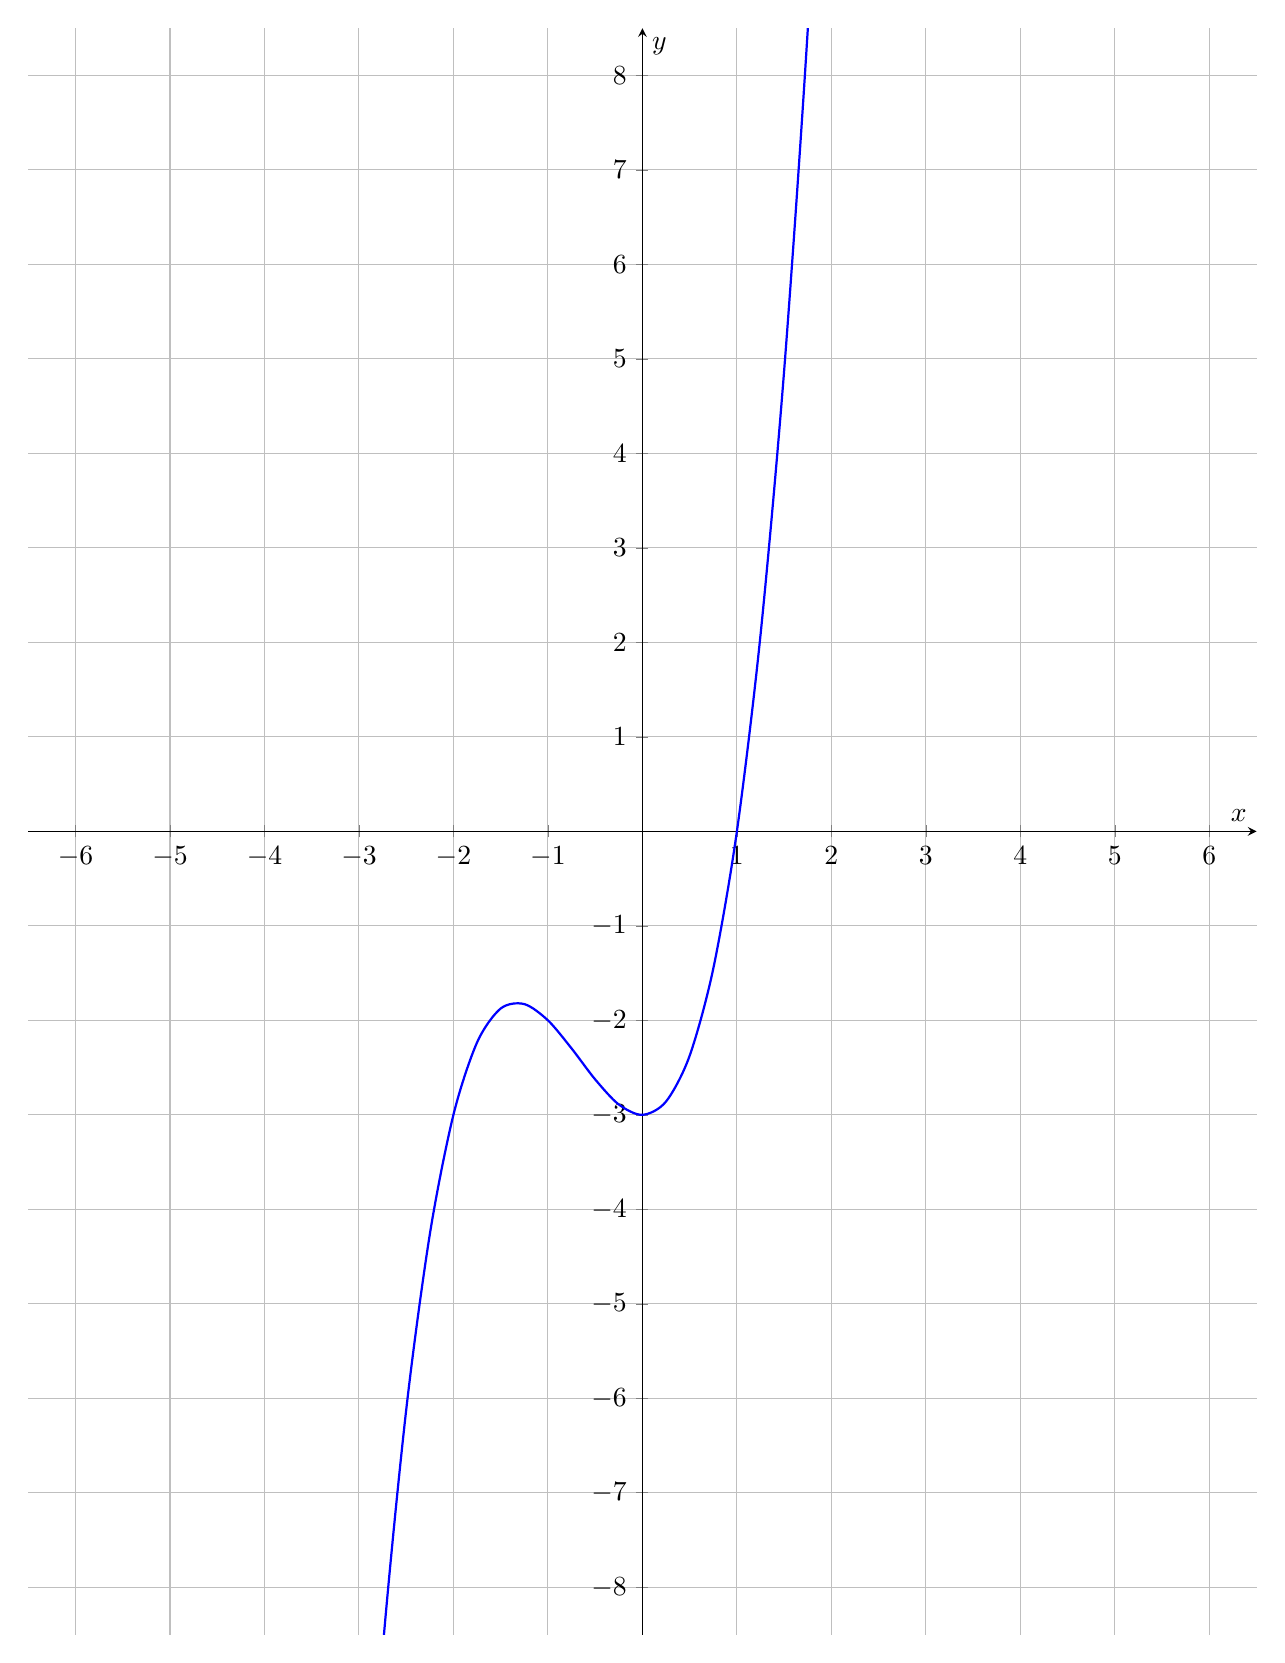
\begin{tikzpicture}
      \begin{axis}[
          xmin = -6.5, xmax = 6.5,
          ymin = -8.5, ymax = 8.5,
          xtick distance = 1.0,
          ytick distance = 1.0,
          x = 1.2cm,
          y = 1.2cm,
          major grid style = {lightgray},
          minor grid style = {lightgray!25},
          grid = both,
          width = \textwidth,
          %height = \textwidth,
          axis x line=center,
          axis y line=center,
          xlabel = {$x$},
          ylabel = {$y$},
        ]
          \addplot[
              domain = -3:3,
              smooth,
              thick,
              blue,
          ] {x^3+2*x^2-3};
          \addplot[
              domain = -2:3,
              smooth,
              thick,
              red,
              answer plot,
          ] {7*x-7};
          \addplot[
              domain = 1:2,
              smooth,
              thick,
              green,
              answer plot,
          ] {0};
          \addplot[
              domain = 0:7,
              smooth,
              thick,
              green,
              answer plot,
          ] (2,x);
      \end{axis}
    \end{tikzpicture}
  \end{center}
    \begin{parts}
      \part
      Differenzieren Sie die Funktion $f(x)$ zeichnerisch bei $x=1$.
      \part
      Differenzieren Sie die Funktion $f(x)$ rechnerisch im Punkt $P_1(1;0)$.
      \begin{solution}
        \begin{enumerate}
          \item Zweiten Punkt der Sekante durch $P_1$ bestimmen:
            \[ P_2(1+h;f(1+h)) \]
            mit
            \[ f(1+h) = h^3+5h^2+7h \]
          \item Steigung der Sekante bestimmen (Differenzenquotient):
            \[
              \begin{aligned}
                m_s &= \frac{\Delta f(x)}{\Delta x} \\
                &= \frac{f(x_2)-f(x_1)}{x_2-x_1} \\
                &= \frac{h^3+5h^2+7h - 0}{1+h - 1} \\
                &= \frac{h^3+5h^2+7h}{h} \\
                &= h^2+5h+7
              \end{aligned}
            \]
          \item Steigung der Tangente durch Annäherung der Punkte mit $h \to 0$ (Differenzialquotient):
            \[
              \lim \limits_{h \to 0} m_s = 0 + 0 + 7 = 7
            \]
        \end{enumerate}
      \end{solution}
      \part
      Differenzieren Sie die Funktion $f(x)$ allgemein, d. h. an einer beliebigen Stelle $x$.
      \begin{solution}
        Bestimmen der Ableitungsfunktion $f'(x)$:
        \[
          f'(x) = 3x^2 + 4x
        \]
      \end{solution}
    \end{parts}

    \question
    Gegeben Sei die folgende Funktion \[ f(x) = \frac{2x+1}{x^2} \]
    \begin{parts}
      \part
      Bestimmen Sie die Ableitungsfunktion $f'(x)$.
      \begin{solution}
        Ableitung mittels Produktregel:
        \[
          \begin{aligned}
          f(x) &= (2x+1)(x^{-2}) = u(x) \cdot v(x) \\
            f'(x) &= u'(x)\cdot v(x) + u(x)\cdot v'(x) \\
            &= 2x^{-2} - (2x+1)2x^{-3} \\
            &= -2 \left(\frac{2x+1}{x^3} \right) + \frac{2}{x^2}
          \end{aligned}
        \]
      \end{solution}
      \part
      Berechnen Sie den Anstieg der Funktion $f(x)$ an der Stelle $x=-\frac{1}{2}$.
      \begin{solution}
        Berechnen von
        \[
          f'(-\frac{1}{2}) = 8
        \]
      \end{solution}
    \end{parts}

    \question
    Gegeben Sei die Funktion $f(x) = \sqrt{x^2+1}$.
    \begin{parts}
      \part
      Bestimmen Sie die Ableitungsfunktion $f'(x)$.
      \begin{solution}
        \[
          \begin{aligned}
            f(x) &= (x^2+1)^{\frac{1}{2}} \\
            &= g(x)^{\frac{1}{2}} \\
            f'(x) &= \frac{1}{2} \cdot g(x)^{-\frac{1}{2}} \cdot g'(x) \\
            &= \frac{2x}{2\sqrt{x^2+1}} \\
            &= \frac{x}{\sqrt{x^2+1}}
          \end{aligned}
        \]
      \end{solution}
    \end{parts}

    \question
    Gegeben Sei die Funktion $f(x)=|x^2-2|-x$.\hfill (*)
    \begin{parts}
      \part
      Ermitteln Sie, ob die Funktion an allen Stellen differenzierbar ist.
      \begin{solution}
        $f(x)$ nicht überall differenzierbar, da sie Knickstellen aufweist:
        \[
          \begin{aligned}
            x^2 - 2 = 0 \\
            x_1 = 0 + \sqrt{2} = \sqrt{2} \\
            x_2 = -\sqrt{2}
          \end{aligned}
        \]
      \end{solution}
      \part
      Bestimmen Sie die Ableitungsfunktion von $f(x)$.
      \begin{solution}
        Bestimmen der abschnittsweise definierten Teilfunktionen mittels Fallunterscheidung:\\
        Fall 1:
        \[
          \begin{aligned}
            x^2 - 2 < 0 \\
            x^2 < 2 \\
            x < \sqrt{2} \land x > -\sqrt{2} \\
            f_1(x) = -x^2+2-x
          \end{aligned}
        \]
        Fall 2:
        \[
          \begin{aligned}
            x^2 - 2 \geq 0 \\
            x^2 \geq 2 \\
            x \geq \sqrt{2} \land x \leq -\sqrt{2} \\
            f_2(x) = x^2-2-x
          \end{aligned}
        \]
        $\Rightarrow$
        \[
          f(x) = \left\{ 
            \begin{array}{ll}
              x^2-x-2 & \text{für } x \geq \sqrt{2} \land x \leq -\sqrt{2} \\
              -x^2-x+2 & \text{für } -\sqrt{2} < x < \sqrt{2}
            \end{array}
          \right.
        \]
        Differenzieren der Teilfunktionen:
        \[
          f(x) = \left\{ 
            \begin{array}{ll}
              2x-1 & \text{für } x \geq \sqrt{2} \land x \leq -\sqrt{2} \\
              -2x-1 & \text{für } -\sqrt{2} < x < \sqrt{2}
            \end{array}
          \right.
        \]
      \end{solution}
    \end{parts}

\end{questions}

\end{document}
